%-------------------------------------------------------------------------------------------------------------------
%        FS-TARMA Models for Non-stationary Vibration Analysis: An overview and comparison
%-------------------------------------------------------------------------------------------------------------------
%					Structural Mechanics Group, ETH Zurich
%-------------------------------------------------------------------------------------------------------------------
%	                          ICOSSAR 2013
%-------------------------------------------------------------------------------------------------------------------
\documentclass[10pt,xcolor = dvipsnames]{beamer} 
\usecolortheme[cmyk={0.05,0.95,.94,0.6}]{structure} 

\usetheme{Warsaw}

\usepackage{latexsym,mathrsfs,amsfonts,pifont}
\usepackage{amsmath,amssymb,amsbsy,mathptmx}
\usepackage{setspace,arydshln,multirow}
\usepackage{graphicx,color}
\usepackage{helvet}
\usepackage{pgfpages}
\usepackage{tikz} 

\usetikzlibrary{arrows,shapes}

\tikzstyle{every picture}+=[remember picture]
\tikzstyle{na} = [baseline=-.5ex]
\tikzstyle{block}=[draw opacity=0.7,line width=1.4cm]

\AtBeginDvi{\special{papersize=297mm,210mm}}

\AtBeginSection[\tableofcontents]

\defbeamertemplate*{footline}{mytheme}
{
  \leavevmode%
  \hbox{%
  \begin{beamercolorbox}[wd=.25\paperwidth,ht=2.25ex,dp=1ex,center]{author in head/foot}%
    \usebeamerfont{author in head/foot}\insertshortauthor
  \end{beamercolorbox}%
  \begin{beamercolorbox}[wd=.525\paperwidth,ht=2.25ex,dp=1ex,center]{title in head/foot}%
    \usebeamerfont{title in head/foot}\insertshorttitle
  \end{beamercolorbox}%
  \begin{beamercolorbox}[wd=.225\paperwidth,ht=2.25ex,dp=1ex,right]{date in head/foot}%
    \usebeamerfont{date in head/foot}\insertshortdate{}\hspace*{2em}
    \insertframenumber{} / \inserttotalframenumber\hspace*{2ex} 
  \end{beamercolorbox}}%
  \vskip0pt%
}


\beamertemplateballitem
\beamertemplatetransparentcovereddynamic

\setbeamertemplate{blocks}[rounded][shadow=true] 

\setbeamercovered{transparent}

\usefonttheme{professionalfonts}

\useoutertheme{default}

\setbeamertemplate{navigation symbols}%[]{}

\setbeamertemplate{caption}[numbered]

\setbeamerfont*{frametitle}{size=\normalsize,series=\bfseries}

\setbeamerfont*{headline}{size*={6}{1}} % shape=\scshape

\setbeamerfont*{footline}{size*={6}{1}}

\setbeamerfont{block title}{size=\normalsize}

\setbeamerfont*{caption}{size=\scriptsize}

\setbeamerfont{math text}{family=\rmfamily}

\setbeamersize{text margin left = 3ex} 

\setbeamersize{text margin right = 3ex} 

\graphicspath{{figures/}}


%------------------------------------------------------------------------------------------------------------
%------------------------------------------------------------------------------------------------------------
%                                             PREAMBLE
%------------------------------------------------------------------------------------------------------------
%------------------------------------------------------------------------------------------------------------
\newcommand{\bc}{\begin{center}}
\newcommand{\ec}{\end{center}}
\newcommand{\noin}{\noindent}
\newcommand{\vc}[1]{\vspace*{#1cm}}
\newcommand{\hc}[1]{\hspace*{#1cm}}
\newcommand{\beq}{\begin{equation}}
\newcommand{\eeq}{\end{equation}}


%------------- list of symbols--------------
\newcommand{\df}{\stackrel{\Delta}{=}}
\newcommand{\bop}{\mathcal{B}}
\newcommand{\sw}{\sigma^2_w[t]}
\newcommand{\M}{\mathcal{M}}
\newcommand{\bth}{\bld{\theta}}
\newcommand{\bPhi}{\bld{\Phi}}
\newcommand{\bphi}{\bld{\phi}}
\newcommand{\bPsi}{\bld{\Psi}}
\newcommand{\bpsi}{\bld{\psi}}
\newcommand{\bvth}{\bld{\vartheta}}
\newcommand{\bld}[1]{\mbox{\boldmath $#1$}}
\newcommand{\E}[1]{\texttt{E}\left\{#1\right\}}
\newcommand{\x}{\bld x}
\newcommand{\e}{\bld e}
\newcommand{\s}{\bld s}
\newcommand{\bz}{\bld{z}}
\newcommand{\Cov}{\bld \Sigma}
\newcommand{\bxi}{\bld{\xi}}

%------------- list of colors --------------
\newcommand{\Blue}{\color{blue}}
\newcommand{\Red}{\color{red}}
\newcommand{\Green}{\color{green}}
\newcommand{\Black}{\color{black}}
\newcommand{\Magenta}{\color{magenta}}
\newcommand{\Brown}[1]{\textcolor[rgb]{0.50,0.25,0.00}{#1}}
\definecolor{gray}{rgb}{0.6,0.6,0.6}
\newcommand{\Gray}{\color{gray}}
\definecolor{QQ}{cmyk}{0.7,0.1,0.9,0.6}
\newcommand{\QQ}{\color{QQ}}
\newcommand{\Redunder}[1]{{\color{red}\underline{\Black{#1}}}}
\newcommand{\Blueunder}[1]{{\color{blue}\underline{\Black{#1}}}}
% ETH logo
\newcommand{\CIMimage}{
\includegraphics[height=6ex]{figures/eth-deutsch.jpg}}



\title[Metamodeling of Structural Systems with Parametric Uncertainty]{\large Metamodeling of Structural Systems with Parametric Uncertainty Subject to Stochastic Excitation}
\author[M.D. Spiridonakos, N.E. Chatzi]{{\bf M.D. Spiridonakos, N.E. Chatzi}\\[1.5ex]
Institute of Structural Engineering,\\ Department of Civil, Environmental \& Geomatic Engineering,\\ ETH Zurich}

\date{\tiny ICOSSAR 2013}{}


\begin{document}
%----------------------------------------------------------
%----------------------------------------------------------
% 				Title (page 1)
%----------------------------------------------------------
%----------------------------------------------------------
 \frame{

\begin{beamercolorbox}[wd=0.9\paperwidth,ht=1.025ex,dp=1.125ex,ignorebg,leftskip=-.1cm,rightskip=14cm]{section in head/foot}
\usebeamerfont{section in head/foot}%
\hskip 6pt\insertsectionhead\hfill\raisebox{-0.8cm}[0pt]{\CIMimage}
% <--- logo is placed here.
\end{beamercolorbox}


\titlepage
\vspace{-.7in}
\begin{figure}
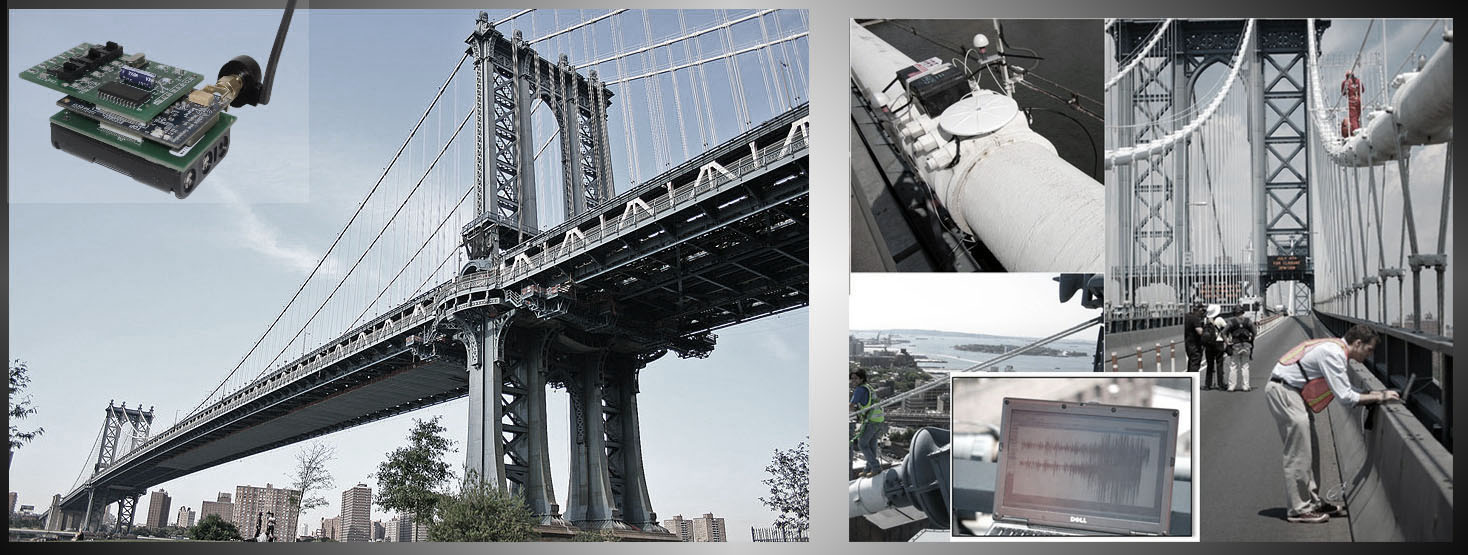
\includegraphics[width=2.5in]{figures/poster2.jpg}
\end{figure}

\vc{0.3}\bc {\small \bf 11th International Conference on Structural Safety \& Reliability} \\
{\footnotesize \bf ICOSSAR 2013}\ec
}




%----------------------------------------------------------
%----------------------------------------------------------
%              Talk Outline (page 2)
%----------------------------------------------------------
%----------------------------------------------------------
\begin{frame}[t]{Talk Outline}

\vc{0.3}
\begin{block}{\large \bf Talk Outline}
\begin{enumerate}
\large\itemsep 15pt
\item{Introduction}
\item PC-NARX metamodels
%\begin{itemize}
%	\item{Parameter estimation}
%	\item{Structure selection}
%\end{itemize}
\item{Numerical Case Study}
\item{Concluding Remarks \& Outlook}
\end{enumerate}
\end{block}

\end{frame}

\clearpage



%----------------------------------------------------------
%----------------------------------------------------------
%              Introduction (page 3)
%----------------------------------------------------------
%----------------------------------------------------------
\begin{frame}[t]{1. Introduction}

\vc{-0.3}\begin{block}{Background \& motivation}
\small Simulation models are extensively used in civil engineering practice. Such models allow the user to 
\begin{itemize}
\item{{\Red understand} structural system performance,}
\item{{\Blue predict} structural behavior,}
\item{{\Red diagnose} damage,}
\item{{\Blue optimize} design, etc}
\end{itemize} 
without ``threatening'' the integrity of the structure. Yet, in a lot of cases realistic excitation is either {\Red unrealizable} or too {\Red costly}. 
\end{block}



\vc{-0.1}\begin{block}{}

\begin{figure}[t!]
\centering
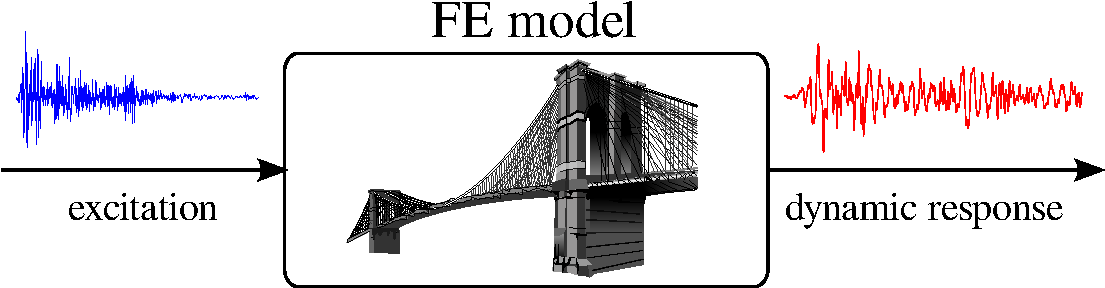
\includegraphics[height = 60pt]{dynamic.pdf}
\end{figure}

\vc{-0.2}\small The simulation of {\Blue dynamic response} through FE models requires {\Red excessive computational resources} particularly for complex, large structures.
 
\end{block}

\end{frame}



%----------------------------------------------------------
%----------------------------------------------------------
% Introduction - Problem characteristics  (page 4)
%----------------------------------------------------------
%----------------------------------------------------------
\begin{frame}{1. Introduction}

\vc{-0.3}

{\bf Problem characteristics}

\vc{-0.2}\begin{columns}
%
\column{0.48\textwidth}

\begin{block}{\small Structural system is characterized by parameter uncertainty}

\begin{figure}[t!]
\centering{
\begin{picture}(150,105)
	\put(0,15){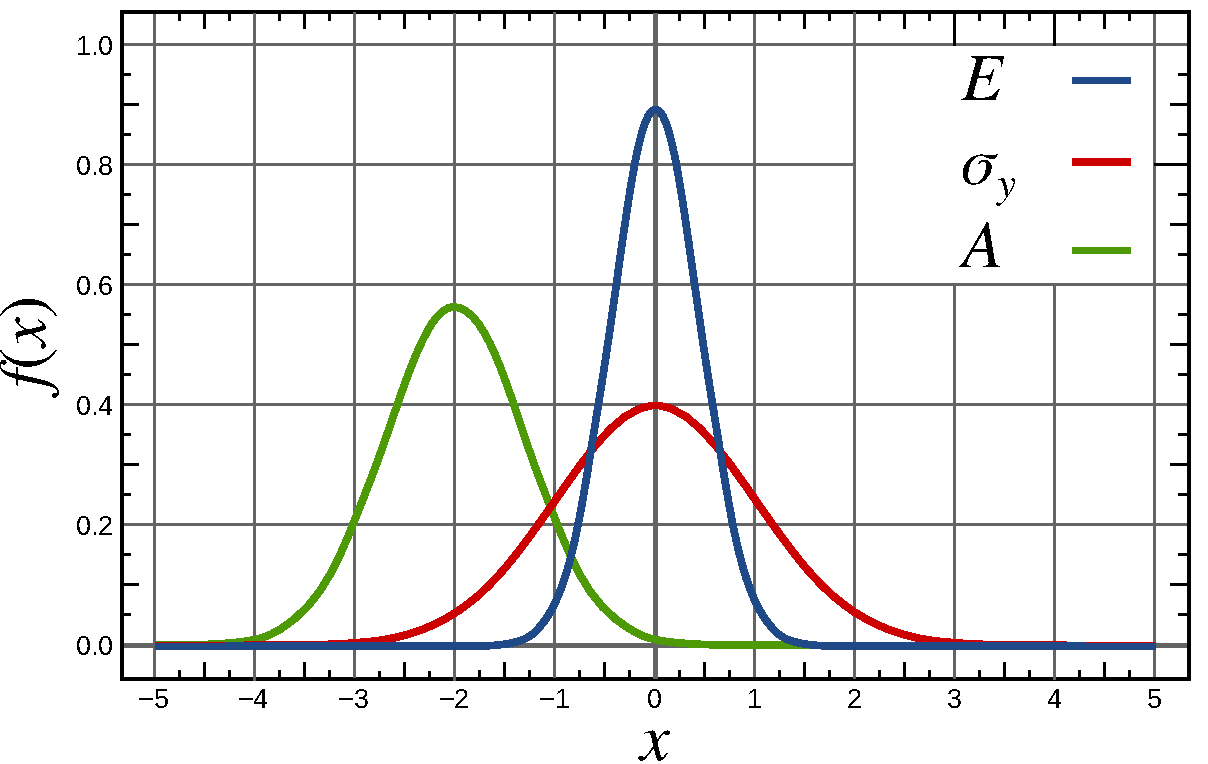
\includegraphics[width = 145pt]{uncertain.pdf}}	
	\put(71,-10){
\includegraphics[height = 20pt]{arrow.pdf}}	
\end{picture}}
\end{figure}

\small \centering The behaviour of the modelled structure has to be examined for a {\Red range of structural characteristics}.

\end{block}

\column{0.48\textwidth}

\begin{block}{\small Nonlinearities are taken into account}

\begin{figure}[t!]
\centering{
\begin{picture}(150,125)
	\put(0,22){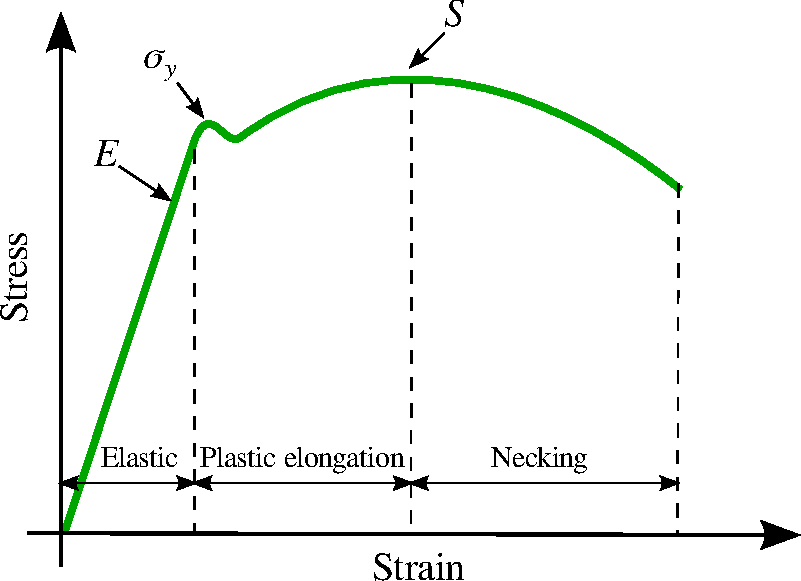
\includegraphics[width = 145pt]{material.pdf}}	
	\put(65,-5){
\includegraphics[height = 20pt]{arrow.pdf}}	
\end{picture}}
\end{figure}
%
\small \centering The impact of {\Red different types of excitation} (of different magnitude and/or spectral content) should also be examined.

\end{block}

\end{columns}


\end{frame}



%----------------------------------------------------------
%----------------------------------------------------------
%  Introduction - Metamodeling problem (page 5)
%----------------------------------------------------------
%----------------------------------------------------------
\begin{frame}{1. Introduction}

{\bf The metamodeling problem}

\begin{figure}[t!]
\hc{-0.4}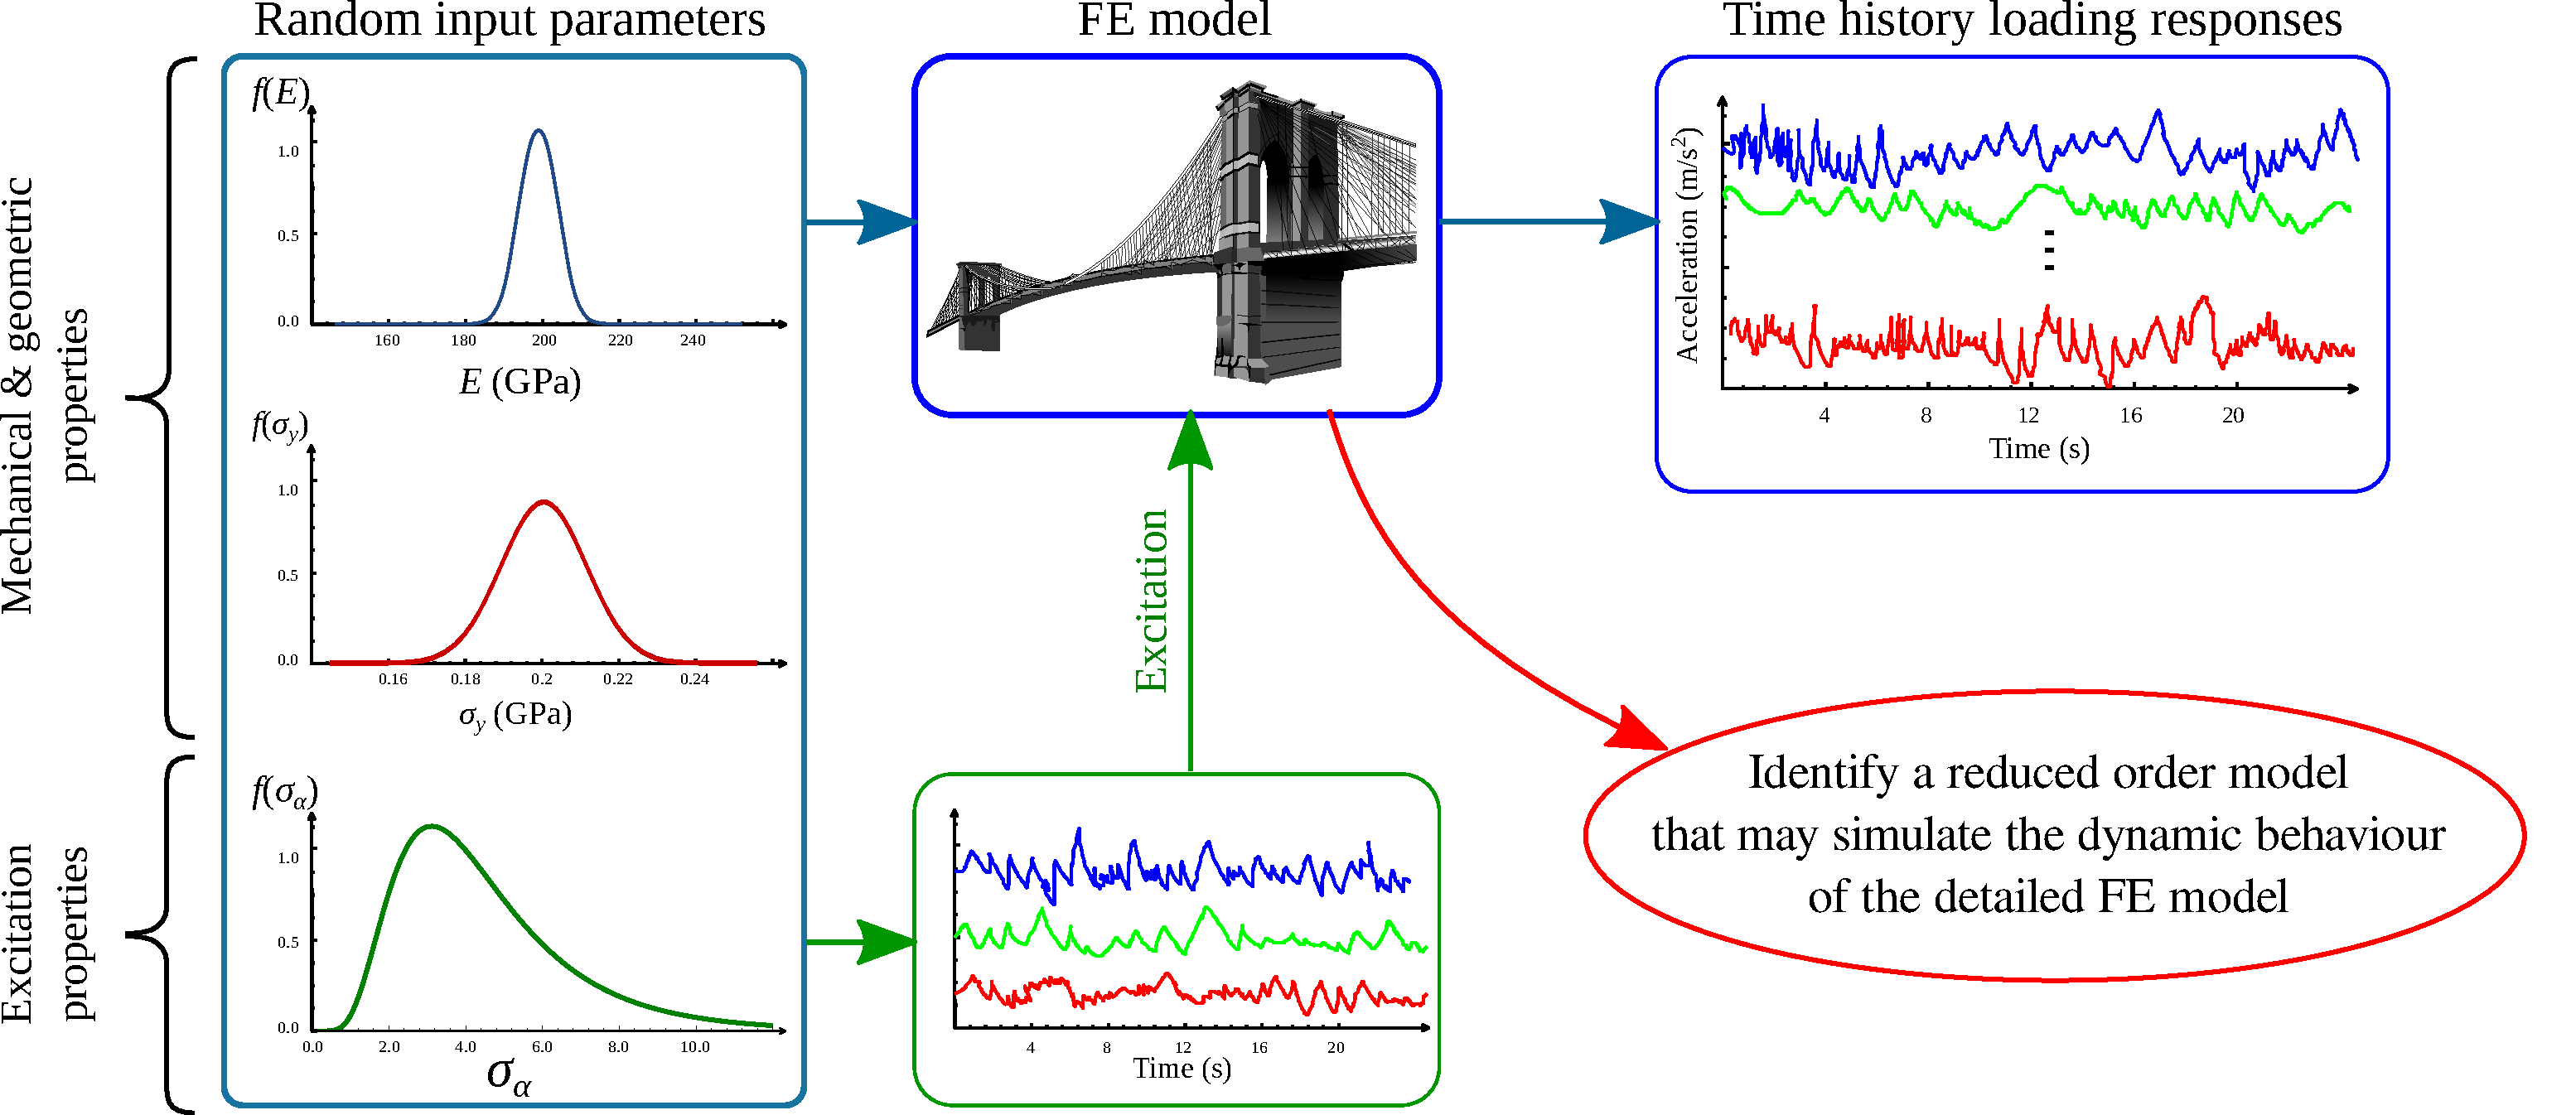
\includegraphics[width = 1.1\textwidth]{FEMsimulations.pdf}
\end{figure}



\end{frame}


%----------------------------------------------------------
%----------------------------------------------------------
% Introduction - Problem definition (page 6)
%----------------------------------------------------------
%----------------------------------------------------------
\begin{frame}{1. Introduction}

\vc{-0.2}\begin{block}{Problem definition}

\bc\small Consider a structural system represented by a numerical model $\cal M$ characterized by uncertain input parameters $\bxi= [ \xi_1, \xi_2,\ldots ,\xi_M ]^{\mathsf T}$ with known joint pdf $f(\bxi)$. The {\Red dynamic response of $\cal M$} to a given input excitation $x[t,\bxi]$  will also be a {\Blue random variable}:
%%
$$ y[t,\bxi] = {\cal M}(x[1,\bxi],x[2,\bxi],\ldots,x[t,\bxi],\bxi), \quad t = 1,2,\ldots, T$$
%%

A {\Red metamodel {$\tilde{\cal M}$}} which must be able to predict and/or simulate the detailed numerical model results in a computationally inexpensive way and with sufficient accuracy is sought.
\ec

\end{block}


\vc{-0.1}\begin{block}{Objectives of the study}
\vc{0.1}{\small \begin{itemize}
\itemsep 0pt
\item{Development of a {\Red metamodeling method} based on PC-NARX models}
\item{Introduction of {\Blue PC-NARX identification methods} for both {\Red prediction} and {\Red simulation} purposes.}
\item{The {\Red validation} of PC-NARX metamodeling method through its application to the case of a {\Blue five-storey shear frame} model subjected to dynamic excitation leading to {\Blue nonlinear response}.}
\end{itemize}}
\end{block}

\end{frame}


%----------------------------------------------------------
%----------------------------------------------------------
% PC-NARX models - Definition (page 7)
%----------------------------------------------------------
%----------------------------------------------------------
\begin{frame}{2. PC-NARX models}

\tikzstyle{every picture}+=[remember picture]
\tikzstyle{na} = [baseline=-.5ex]

\vc{-0.3}\begin{block}{Polynomial Chaos Nonlinear ARX (PC-NARX) models}
%
\vc{-0.1}$$\Red\boxed{\Black \quad y[t] =  \sum_{i=1}^{n_\theta} \theta_i(\bxi) \cdot g_i({\bld z}[t]) + e[t]   \quad }$$

\vc{-2}\begin{figure}[t!]
\centering{
\begin{picture}(300,1)(0,42)
\put(120,0){
\begin{tikzpicture}[>=triangle 45,line width=.02cm]
\Red \draw[->] ( 0, 0) -- ( -0.7, -0.7);
\draw[->] ( 1.0, 0) -- (3.5, -0.9);
\end{tikzpicture}}
\end{picture}}
\end{figure}

\vc{0.5}

\begin{columns}

\column{0.6\textwidth}
\begin{equation*}
\tikz[baseline]{
       	     \node[fill=red!20, ellipse,anchor=base] ()
            {\begin{minipage}[h]{5cm}{\bc \vc{-0.2}\footnotesize random parameters $\theta_i(\bxi)$ describe the uncertainty propagation.  They may be expanded on a PC basis orthogonal to the pdf of the random input variables $\bxi$ $$ 
\theta_i (\bxi) = \sum_{j=1}^{p } \theta_{i,j}\cdot \phi_{\bld{d}(j)}(\bxi) $$ \vc{-0.6} \ec} \end{minipage}};}
\end{equation*}

\column{0.35\textwidth}
\begin{equation*}
\tikz[baseline]{
       	     \node[fill=red!20, ellipse,anchor=base] ()
            {\begin{minipage}[h]{2.5cm}{\bc \footnotesize $g_i (\cdot)$: nonlinear function operators that reflect the nonlinear structural dynamics \vc{-0.1} \ec} \end{minipage}};}
\end{equation*}
\end{columns}

\begin{columns}

\column{0.45\textwidth}

\tiny 
\begin{tabular}{l}
{\Red ${\bld z}[t] = \bigl[ y[t-1],$ $\ldots, y[t-n_a], $ $x[t],\ldots ,x[t-n_b] \bigr]^\mathsf{T}$}: regression vector \\
 {\Red $n_a, n_b$}: maximum output and input time lags  \\  
{\Red $e[t]$}: residual sequence \\
{\Red $\theta_{i,j}$}: unknown deterministic coefficients of projection \\
{\Red ${\bld d}{(j)}$}: multi-indices of the multivariate polynomial basis \\ 
\end{tabular} 

\begin{block}{\small PC-NARX parameter estimation}
\begin{itemize}
\item{\footnotesize coefficients of projection $\theta_{i,j}$}
\end{itemize}
\end{block}
\vc{1.25}
\column{0.45\textwidth}

\tiny 
\begin{tabular}{l}
{\Red $n_\theta$}: number of nonlinear regression terms \\  
{\Red $\sigma_e^2$}: residual sequence variance \\
{\Red $\phi_{{\bld d}(j)}$}: basis functions orthonormal w.r.t. the joint pdf of $\bxi$ \\ 
\end{tabular} 

\begin{block}{\small PC-NARX structure selection}
\begin{itemize}
\item{\footnotesize select nonlinear functions $g_i(z[t])$ (polynomial, wavelet, radial basis functions, and so on)}
\item{\footnotesize select PC functional subspace}
\end{itemize}
\end{block}
\end{columns}


\end{block}

\end{frame}


%----------------------------------------------------------
%----------------------------------------------------------
% PC-NARX models - PE estimation (page 8)
%----------------------------------------------------------
%----------------------------------------------------------
\begin{frame}{2. PC-NARX models}

\vc{-0.2}\begin{block}{\small Estimation of a PC-NARX model for purposes of prediction}

\begin{columns}
\column{0.95\textwidth}

\vc{-0.3}\begin{block}{}
\small  \bc Consider $K$ simulations conducted with \ec
\vc{-0.3}
{\Blue $\bxi_k = [\xi_{k,1}, \xi_{k,2}, \ldots ,\xi_{k,M}]^{\mathsf T}$}: random input parameter vector realizations

{\Blue $x_k^T = \{ x_k[1,\bxi_k], x_k[2,\bxi_k], \ldots, x_k[T,\bxi_k] \}$}: set of input excitation signals ($k=1,2,\ldots,K$) 
\end{block}
\vc{-1.0}{\Large \Magenta $$ \Downarrow$$}\vc{-0.8}
\begin{block}{}
\bc  \small \vc{-0.5}{\Red $$y_k^T = \{ y_k[1,\bxi_k], y_k[2,\bxi_k], \ldots, y_k[T,\bxi_k] \} \vc{-0.2}$$ }  
corresponding set of the full scale numerical model dynamic responses\\ \scriptsize (assumed to also follow a PC-NARX model)  \ec
\end{block}{}
\vc{-1.0}{\Large \Magenta $$ \Downarrow$$}\vc{-0.8}
\begin{block}{}{\small \bc Estimation of the coefficients of projection $\bth = [\ a_{1,1}, \ldots, a_{n_a,p}  b_{0,1}, \ldots, b_{n_b,p}\, ]^{\mathsf T}$
%
based on the {\Blue minimization} of the {\Blue Prediction Error} criterion: \vc{-0.2}
%
$$ \widehat{\bth} =\arg\min_{\bth} \left\{ \sum_{k=1}^K \sum_{t=1}^T  (y_k[t] - \hat{y}_k[t|t-1])^2 \right\} = \arg\min_{\bth} \left\{ \sum_{k=1}^K \sum_{t=1}^T  e_k^2[t] \right\} \vc{-0.2}$$ 
%
\scriptsize {\Magenta $ \hat{y}_k[t|t-1]$}: PC-ARX model's one-step-ahead prediction 
\ec}
\end{block}
\vc{-1.0}{\Large \Magenta $$ \Downarrow$$}\vc{-0.9}
%
\begin{block}{}
\vc{-0.1}{\small \centering {\Blue Ordinary Least Squares (OLS)} estimator: 
%
$
\Red\boxed{\Black\widehat{\bth} = \bigl(\bPhi^{\mathsf T}(\bxi) \cdot \bPhi(\bxi) \bigr)^{-1} \cdot \bigl( \bPhi(\bxi)^{\mathsf T} \cdot {\bld Y} \bigr)} $ \vc{-0.2}
%
\scriptsize $${\Red \bPhi(\bxi)}: \text{regression matrix} \qquad {\Red Y}: \text{pooled response signal vector}  $$}
%
\end{block}
\vc{0.2}

\end{columns}

\end{block}

\end{frame}

%-------------------------------------------------------------------------------------------------------------------
%-------------------------------------------------------------------------------------------------------------------
%                                             PC-ARX models	
%-------------------------------------------------------------------------------------------------------------------
%-------------------------------------------------------------------------------------------------------------------
\begin{frame}{2. PC-NARX models}

\vc{-0.1}\begin{block}{Estimation of a PC-ARX model for purposes of simulation}

\small 
% Consider again a set $K$ input excitation signals $x_k^T (k = 1, 2, \ldots,K)$. For each $x_k^T$  $\bar{y}_k [t]$ of a PC-ARX($n_a,n_b$) metamodel

\bc The simulated response of a given PC-NARX metamodel may be obtained recursively as:
% 
$$ 
\Red\boxed{\Black \quad \bar{y}_k[t] = \sum_{i=1}^{n_\theta} \theta_i (\bxi_k) \cdot g_i(\bar{\bld z}[t]) , \quad t = 1,2,\ldots, T \quad}
$$
%
{\footnotesize with given initial conditions $\Red\{ \bar{y}_k[1 - n_a], \ldots, \bar{y}_k[0] \}$ and $\Red \{ x_k[1-n_b], \ldots, x_k[0]\}$} \ec

\begin{columns}
\column{0.95\textwidth}
\begin{block}{}
\centering
Estimation of the model coefficients of projection $\bth$ based on the {\Blue minimization} of the {\Red Simulation Error} criterion:
%
$$\widehat{\bth_s} = \arg\min_{\bth_s} \left\{ \sum_{k=1}^K \sum_{t=1}^T  (y_k[t]- \bar{y}_k[t] )^2 \right\}  =\arg\min_{\bth_s} \left\{ \sum_{k=1}^K \sum_{t=1}^T  \varepsilon_k^2[t] \right\}$$
%
\end{block}
\end{columns}
%
\vc{-0.2}{\LARGE \Red $$ \Downarrow$$}\vc{-0.5}
%
\begin{columns}
\column{0.6\textwidth}
\begin{block}{}
\small \bc Iterative {\Blue nonlinear optimization} methods\ec
\end{block}
\vc{0.2}
\end{columns}

\end{block}

\end{frame}



%----------------------------------------------------------
%----------------------------------------------------------
%              Introduction (page 3)
%----------------------------------------------------------
%----------------------------------------------------------
\begin{frame}[t]{2. PC-NARX models}

\vc{-0.3}
\begin{block}{\small Flowchart of the complete identification scheme}
% Figure
% ================================================
\begin{figure}
{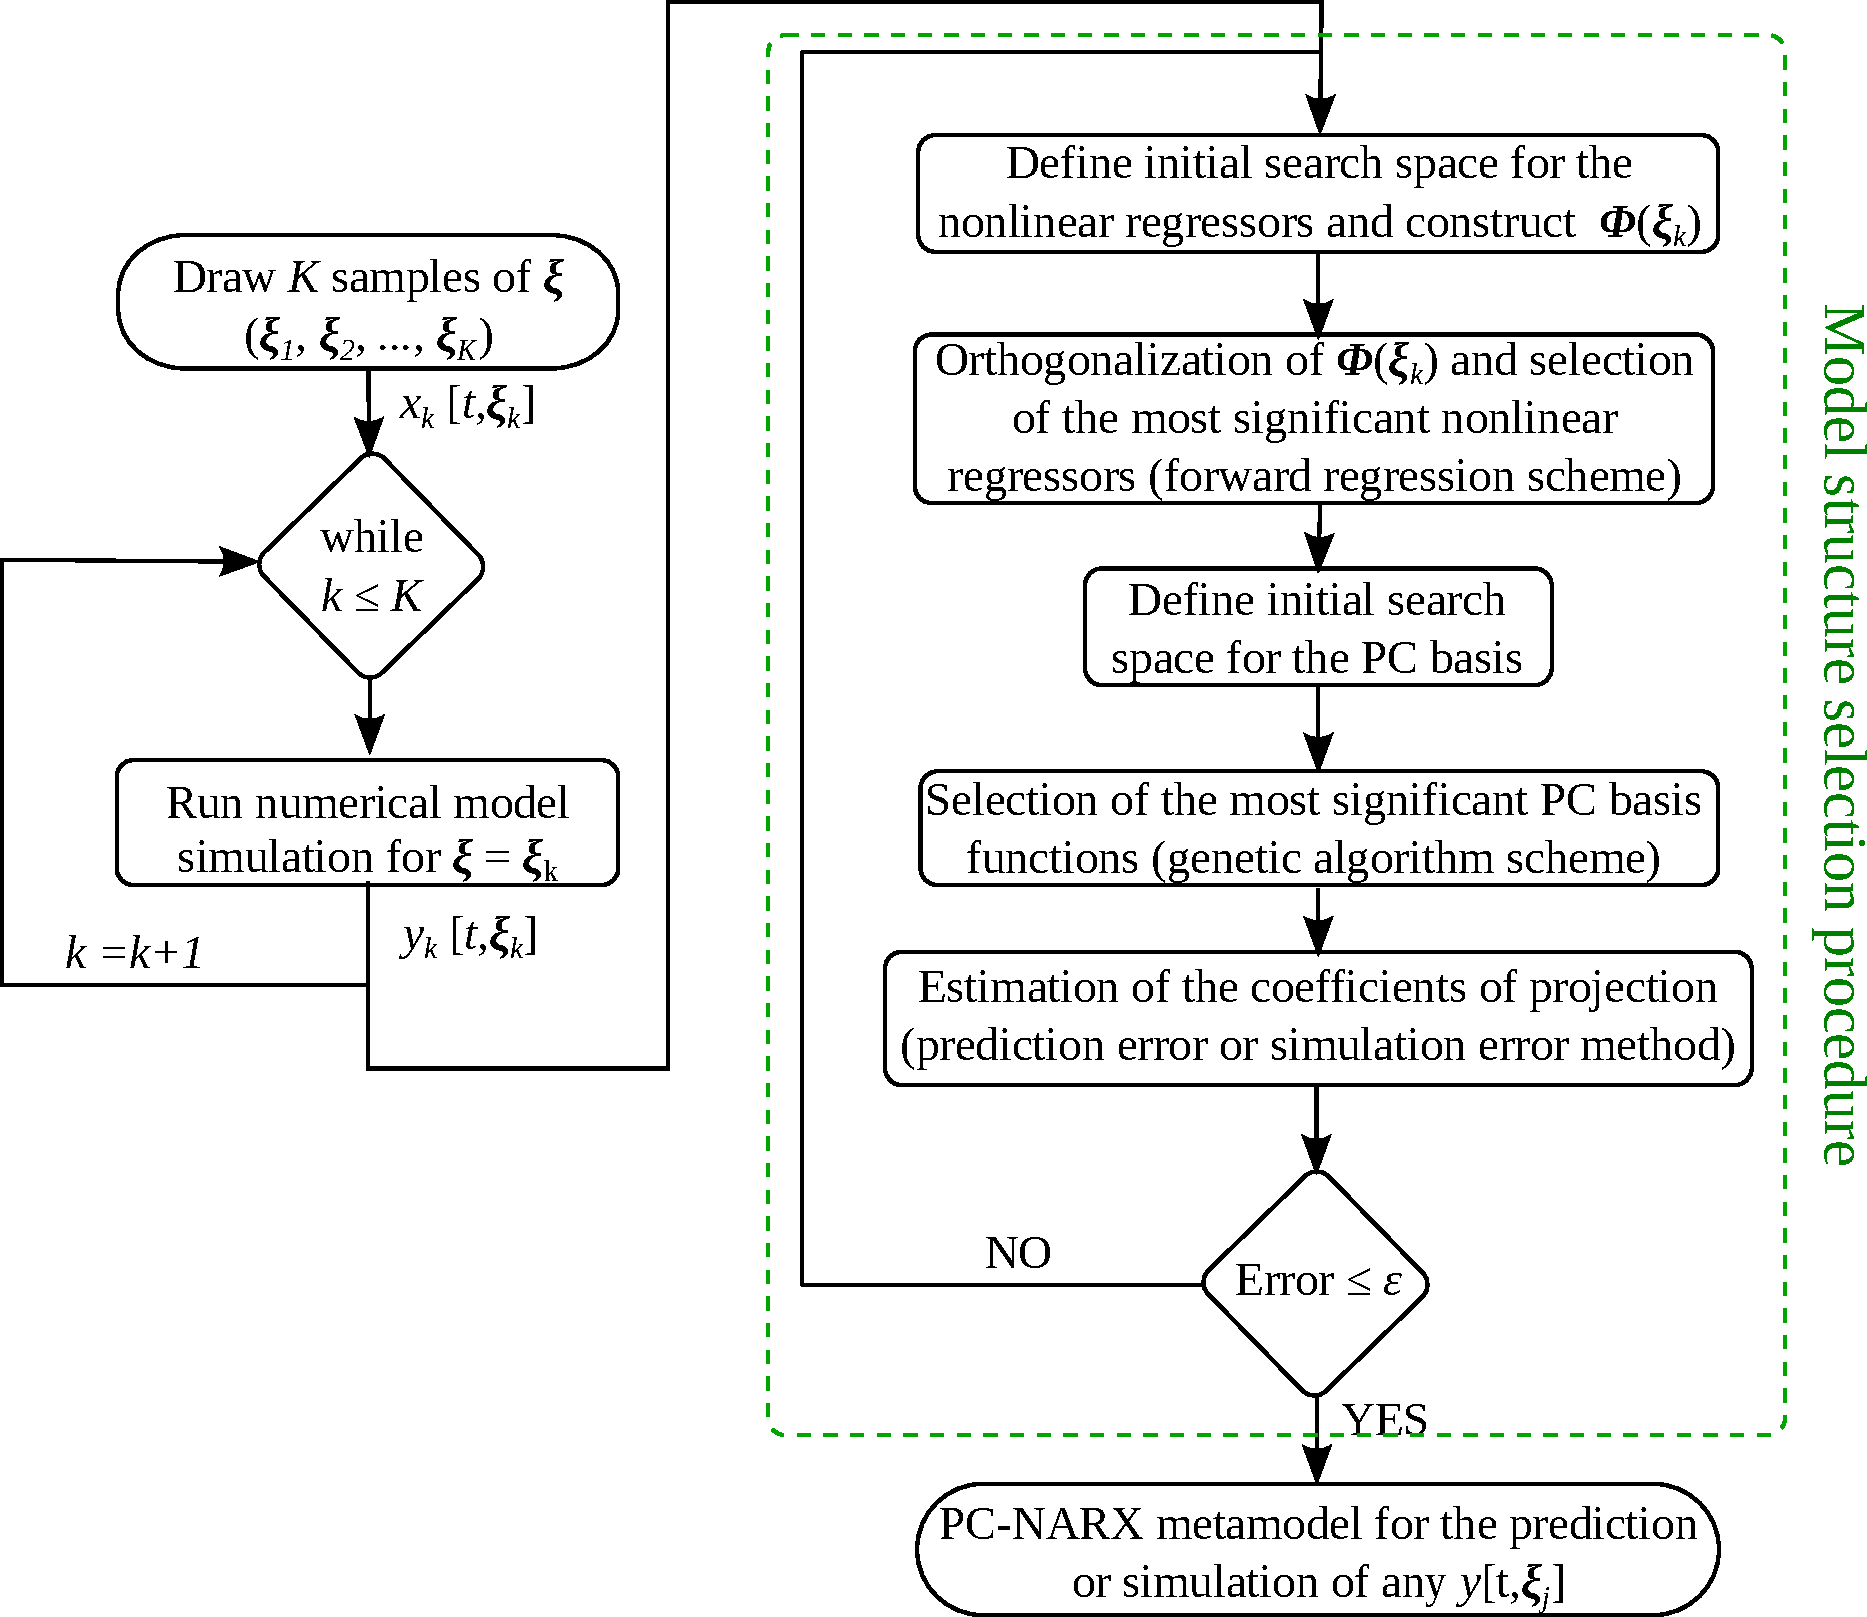
\includegraphics[width=0.75\textwidth]{flowchart.pdf}}
\end{figure}
% ================================================
\end{block}
\end{frame}

%----------------------------------------------------------
%----------------------------------------------------------
%              Introduction (page 3)
%----------------------------------------------------------
%----------------------------------------------------------
\begin{frame}[t]{3. Numerical case study}

\vc{-0.2}{\small \bf A five-storey shear frame model}

\begin{columns}

\column{0.32\textwidth}

% Figure
% ================================================
\begin{figure}[t!]
\includegraphics[width = 0.9\textwidth]{ShearFrame5storey.pdf}
\end{figure}
% ================================================

\column{0.62\textwidth}
% Table
% ================================================
\scriptsize

{\bf Mechanical \& geometric properties}
\begin{spacing}{1.2}
\begin{tabular}{llll}\hline
\multicolumn{2}{l}{Geometric}& \multicolumn{2}{l}{Mechanical}\\[-6pt]
\multicolumn{2}{l}{\hrulefill}& & \\
Cross-sectional area & \hspace{-0.2cm} cm$^2$ & & \\\hline
1$^{\text{st}}$ storey columns & \hspace{-0.2cm} 900 & Poisson ratio & \hspace{-0.2cm} 0.29 \\
2$^{\text{nd}}$ storey columns & \hspace{-0.2cm} 625 & Density (kg/m$^3$)  & \hspace{-0.2cm} 7850\\
3$^{\text{rd}}$ storey columns & \hspace{-0.2cm} 400 & Yield stress (MPa) & \hspace{-0.2cm} 200\\
4$^{\text{th}}$ storey columns & \hspace{-0.2cm} 225 & Tangent modulus (GPa) & \hspace{-0.2cm} 10 \\
5$^{\text{th}}$ storey columns & \hspace{-0.2cm} 100 & & \\ 
Horizontal beams & \hspace{-0.2cm} 100 & & \\\hline
\end{tabular}
\end{spacing}
% ================================================





\end{columns}

\end{frame}



%----------------------------------------------------------
%----------------------------------------------------------
%              Introduction (page 3)
%----------------------------------------------------------
%----------------------------------------------------------
\begin{frame}[t]{3. Numerical case study}
\vc{-0.3}\begin{block}{\small Parametric modelling of earthquake accelerograms\\  \scriptsize \em [S. Rezaeian \& A.D. Kiureghian 2010]}


\begin{figure}[t!]
\centering{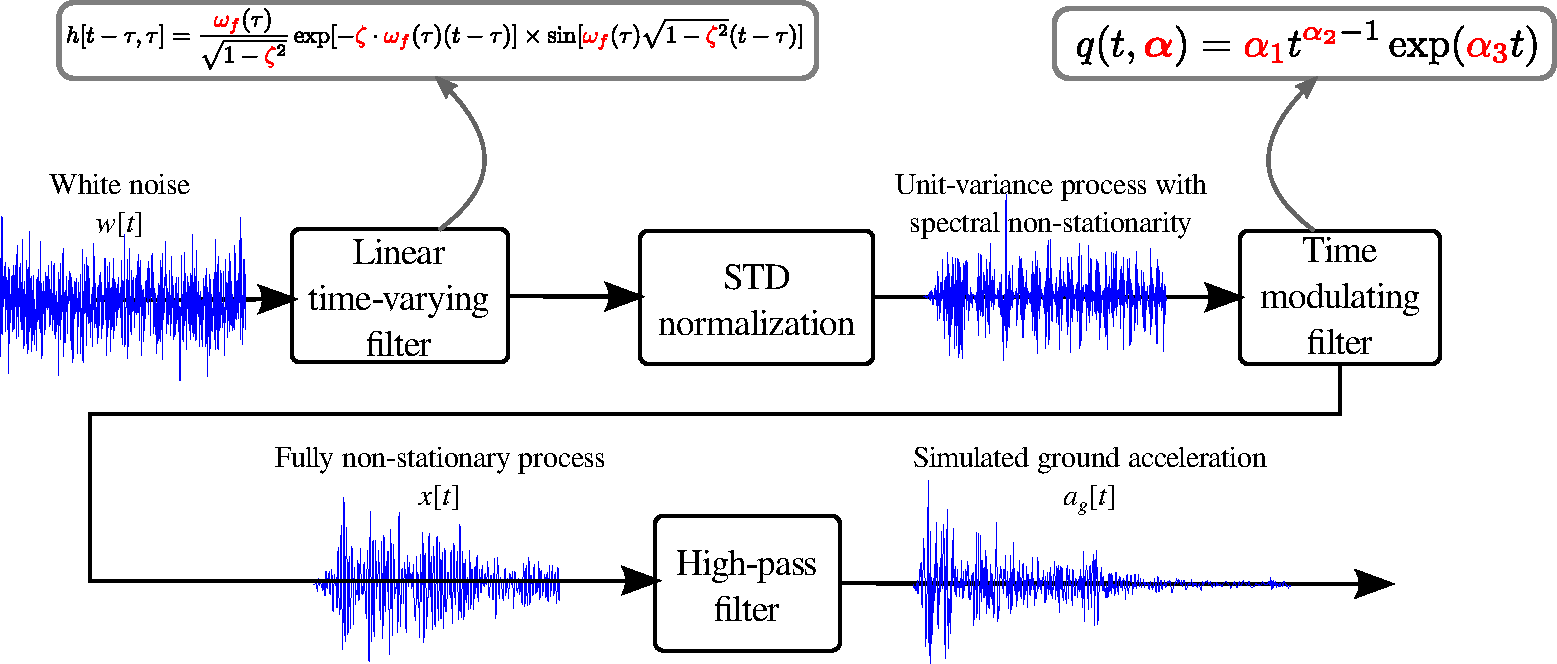
\includegraphics[width=1.0\textwidth]{syntheq.pdf}}
\end{figure}


\begin{columns}
\column{0.4\textwidth}
\scriptsize \begin{tabular}{l} 
{\Blue $\zeta_f$}: damping ratio of the filter \\
{\Blue $\omega_f(\tau) = \omega_{\text{mid}} + \omega'(\tau-t_{\text{mid}})$}: filter's frequency\\
{\Blue $\omega_{\text{mid}}$}: filter frequency at $t_{\text{mid}}$\\
{\Blue $\omega'$}: rate of change of the filter frequency\\
\end{tabular}

\column{0.55\textwidth}

\scriptsize
\scriptsize \begin{tabular}{l} 
{\Blue $\alpha_i$'s}: parameters of the modulating gamma function.  \\ $\qquad$ Directly estimated from:\\
{\Blue $I_a$}: Arias intensity\\
{\Blue $D_{5-95}$ }: effective duration of the motion \\
{\Blue $t_{\text{mid}}$}: time at which 45\% of the Arias intensity is reached\\
\end{tabular}
\end{columns}

\end{block}

\end{frame}



%----------------------------------------------------------
%----------------------------------------------------------
%              Introduction (page 3)
%----------------------------------------------------------
%----------------------------------------------------------
\begin{frame}[t]{3. Numerical case study}

{\small {\bf Modelling of the PEER database accelerograms} \\ \footnotesize (results from the 1000 accelerograms with the best fit)}

% Figure
% ================================================
\begin{figure}
{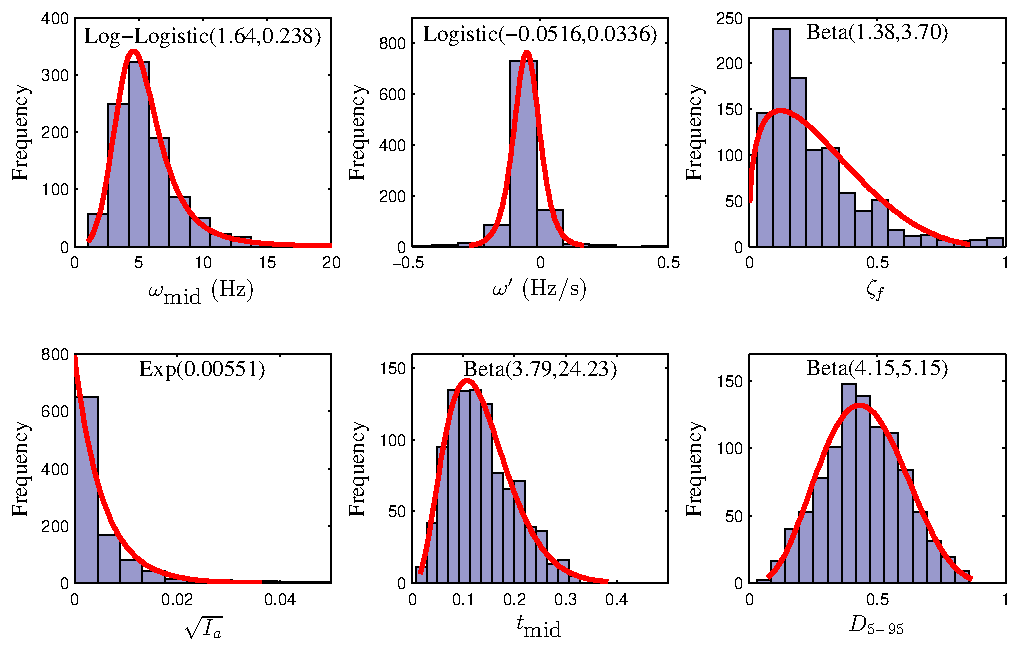
\includegraphics[width=0.95\textwidth]{histfit.pdf}}
\end{figure}
% ================================================

\end{frame}



%----------------------------------------------------------
%----------------------------------------------------------
%              Introduction (page 3)
%----------------------------------------------------------
%----------------------------------------------------------
\begin{frame}[t]{3. Numerical case study}

\vc{-0.2}{\small {\bf Input random vector realizations for the 200 simulations conducted}}

\begin{columns}

\column{0.38\textwidth}

% Table
% ================================================
\vc{-0.1}{\bf \footnotesize Random input variables}
\scriptsize\begin{spacing}{1.2}
\begin{tabular}{lll} \hline 
Variable 	& Distribution 	& pdf parameters \\ [1pt] \hline
\multirow{2}{*}{E (GPa)}  	& \multirow{2}{*}{Uniform} & $\min = 180$  \\
 	&  & $\max = 220$\\ \hdashline
\multirow{2}{*}{$\omega_{\text{mid}}$ (Hz)} & \multirow{2}{*}{Log-Logistic} 	& $\alpha = 1.64 $ \\ & & $\beta = 0.238 $ \\ \hdashline
\multirow{2}{*}{$\omega'$ (Hz/s)} & \multirow{2}{*}{Logistic} 		& $\mu = -0.0516 $ \\ & & $\sigma = 0.0336 $ \\ \hdashline 
$\sqrt{I_a}$ & Exponential & $\mu = 0.00551 $\\ \hdashline
\multirow{2}{*}{$D_{5-95}$} & \multirow{2}{*}{Beta} & $\alpha = 4.15$\\ & & $\beta = 5.15$\\ \hline
\end{tabular}
\end{spacing}
% ================================================


\column{0.65\textwidth}

\vc{-0.2}% Figure
% ================================================
\begin{figure}
\hc{0.7}\centering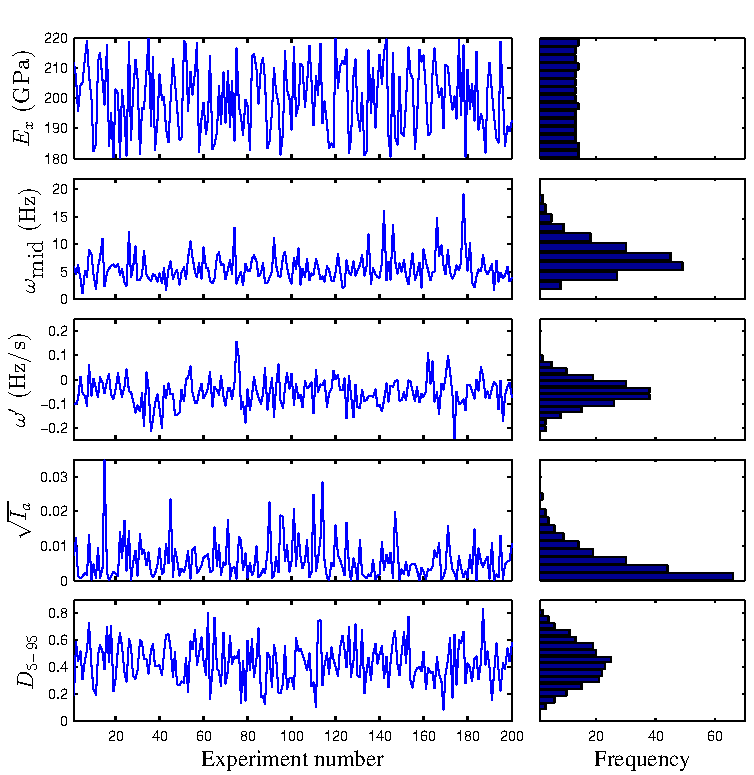
\includegraphics[width=7cm]{input_pars.pdf}
\end{figure}
% ================================================

\end{columns}
\end{frame}


%----------------------------------------------------------
%----------------------------------------------------------
%              Introduction (page 3)
%----------------------------------------------------------
%----------------------------------------------------------
\begin{frame}[t]{3. Numerical case study}

{\small {\bf Input-output data}}

\begin{columns}

\column{0.31\textwidth}

\scriptsize\begin{spacing}{1.2} \begin{tabular}{ll}
\hline
Simulation time  & $T_{\text{sim}} = $ 25 (s)\\
Sampling frequency  & $f_s = $ 40 (Hz)\\
\# of samples  & $T =$ 1000\\
\# of experiments  & $K =$ 200\\
\hline
\end{tabular}
\end{spacing}

\column{0.6\textwidth}
% Figure
% ================================================
\vc{-1.4}\begin{figure}
{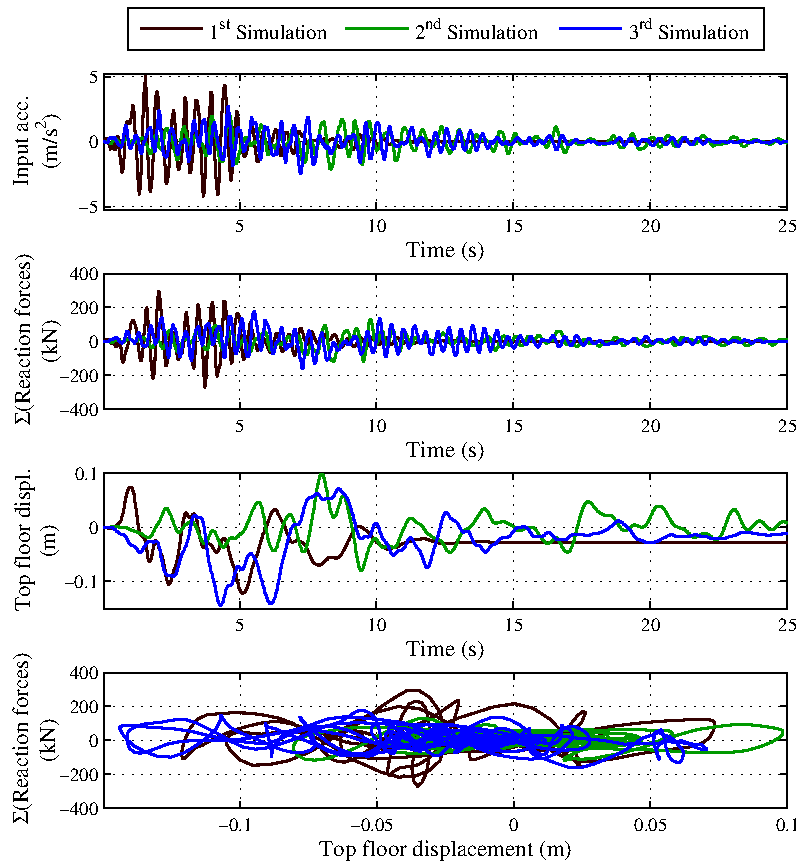
\includegraphics[width=1.05\textwidth]{SF2D_simulations.pdf}}
\end{figure}
% ================================================
\end{columns}

\end{frame}


%----------------------------------------------------------
%----------------------------------------------------------
%              Introduction (page 3)
%----------------------------------------------------------
%----------------------------------------------------------
\begin{frame}[t]{3. Numerical case study}


\vc{-0.3}{\small {\bf PC-NARX identification results}}

\begin{columns}

\column{0.48\textwidth}

\vc{-0.25}\begin{block}{\scriptsize Nonlinear regressors:}
\scriptsize 
{\Blue Initial search space:}

$ g_i({\bld z}[t]) = z_{j_1}^{\ell_1}[t] \cdot z_{j_2}^{\ell_2}[t]$
%
with $\ell_1,\ell_2 = 0,\ldots 3$, $\ell_1 + \ell_2 \leq 3$

${\bld z}[t] = \left[ \ y[t-1], \ldots, y[t-10], x[t], x[t-1], \ldots, x[t-10]\ \right]^{\mathsf{T}}$

{\Blue Finally selected terms:}

$y[t-1], \ldots,y[t-10], x[t], x[t-1], \ldots,x[t-10],$ \vspace{0.2cm} \\
%
$y[t-1]\cdot y^2[t-2], \ldots, y[t-1]\cdot y^2[t-10],$ \vspace{0.2cm} \\
%
$y^2[t-1]\cdot y[t-2], \ldots, y^2[t-1]\cdot y[t-10],$ \vspace{0.2cm} \\
$y^3[t-1], y^3[t-2], y^3[t-3].$
\end{block}

%%
\column{0.44\textwidth}

\vc{-0.25}\begin{block}{\scriptsize
Multi-indices of the selected PC basis functions}
\scriptsize \begin{tabular}{cccccc}\hline
& $E$ & $\omega_{\text{mid}}$ & $\omega'$ & $I_a$ & $D_{5-95}$\\ \hline
${\bld d}{(1)}$ & 0 & 0 & 0 & 0 & 0 \\ 
${\bld d}{(2)}$ & 1 & 0 & 0 & 0 & 0 \\
${\bld d}{(3)}$ & 0 & 1 & 0 & 0 & 0 \\  
${\bld d}{(4)}$ & 0 & 0 & 0 & 0 & 1 \\ 
${\bld d}{(5)}$ & 1 & 0 & 0 & 1 & 0 \\ 
${\bld d}{(6)}$ & 0 & 1 & 0 & 0 & 1 \\ 
${\bld d}{(7)}$ & 0 & 2 & 0 & 0 & 0 \\ 
${\bld d}{(8)}$ & 1 & 2 & 0 & 0 & 0 \\ 
${\bld d}{(9)}$ & 0 & 3 & 0 & 0 & 0 \\ \hline
\end{tabular}
\end{block}
\end{columns}


\vc{0.1}{\small {\bf PC-NARX based prediction and simulation errors}}

\vc{-0.2}
% Figure
% ================================================
\begin{figure}
{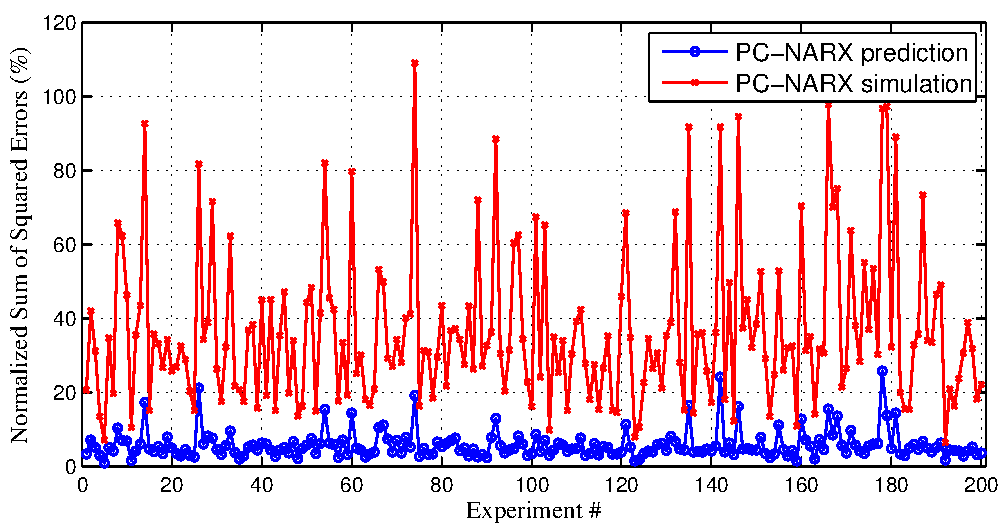
\includegraphics[width=0.65\textwidth]{K_preds_sims.pdf}}
\end{figure}
% ================================================

\end{frame}


%----------------------------------------------------------
%----------------------------------------------------------
%              Introduction (page 3)
%----------------------------------------------------------
%----------------------------------------------------------
\begin{frame}[t]{3. Numerical case study}

{\small {\bf Validation based on a real earthquake ground motion acceleration excitation: FE vs PC-NARX metamodel} \\ \footnotesize (El Centro earthquake time history loading)}

% Figure
% ================================================
\begin{figure}
{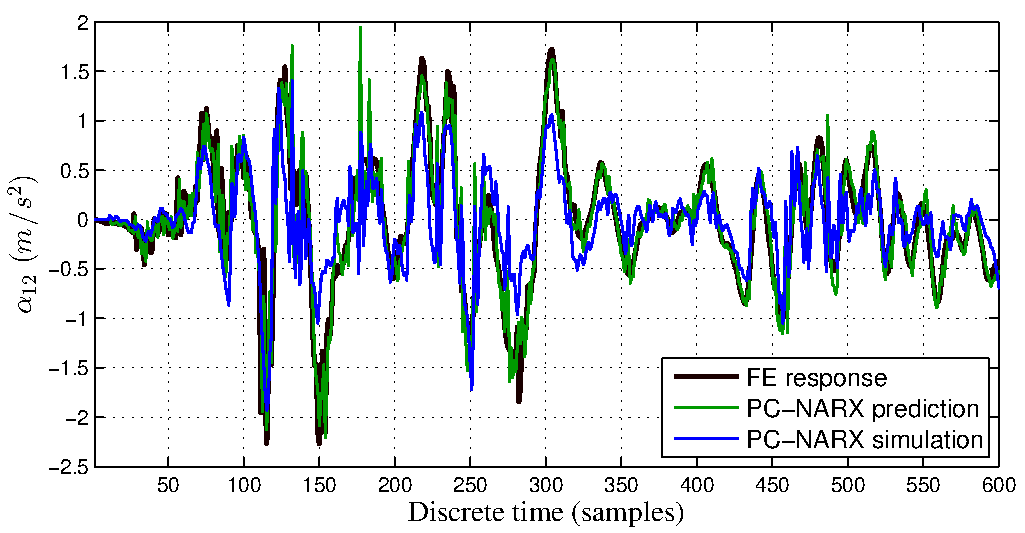
\includegraphics[width=\textwidth]{preds_sims.pdf}}
\end{figure}
% ================================================

{\footnotesize \bf Normalized residual sum of squares: \Red prediction 13.15\%, \Blue simulation 38.10\%  }

\end{frame}




%-------------------------------------------------------------------------------------------------------------------
%-------------------------------------------------------------------------------------------------------------------
%                   Conclusions (page 2)
%-------------------------------------------------------------------------------------------------------------------
%-------------------------------------------------------------------------------------------------------------------
\begin{frame}[t]{4. Concluding Remarks \& Outlook}

\vc{0.1}
\begin{block}{Concluding Remarks}

{\small \begin{itemize}
\itemsep 0pt
\item{Stochastic {\Red metamodels} of low order that are capable of accurately approximating {\Blue FE models} are developed.}
\item{The {\Red metamodeling method} is based on {\Blue Nonlinear ARX} models and {\Blue Polynomial Chaos} basis expansion.}
\item{The numerical results show good {\Blue prediction} and {\Blue simulation} accuracy of the dynamic response of the model.}
\item{The proposed methodology may be adapted as an approximative {\Blue low cost surrogate} for a number of purposes such as {\Red vibration control}, {\Red SHM}, {\Red model updating} and others.}
\end{itemize}}

\end{block}





\end{frame}




%-------------------------------------------------------------------------------------------------------------------
%-------------------------------------------------------------------------------------------------------------------
%                                             PC-basis	
%-------------------------------------------------------------------------------------------------------------------
%-------------------------------------------------------------------------------------------------------------------
\begin{frame}{A. PC basis}

\vc{-0.2}\begin{block}{}

\begin{columns}

\column{0.45\columnwidth}

{\scriptsize The \alert{PC basis} functions $\phi_{{\bld d}(j)}$ are orthonormal with respect to the joint probability density function of $\bxi$:
%%
$$
E[ \phi_{\bld \alpha} (\bxi), \phi_{\bld \beta} (\bxi) ] = \delta_{{\bld \alpha},{\bld \beta}} =\begin{cases} 1 & \mbox{for } \alpha = \beta \\ 0 & \mbox{otherwise} \end{cases}
$$}
%%

\column{0.5\columnwidth}

\vc{-0.5}\begin{center}
{\scriptsize
\begin{tabular}{lcc} \hline
{\bf PDF} & {\bf Support} & {\bf Polynomials} \\
Normal (Gaussian) & $(-\infty,\infty)$ & Hermite \\
Uniform & $[-1, 1]$ & Legendre\\
Gamma & (0,1) & Laguerre \\
Chebyshev & (-1, 1) & Chebyshev\\
Beta & (-1, 1)& Jacobi\\ \hline
\end{tabular}}
\end{center}
\end{columns}
\vc{-0.2}
\end{block}

\vc{-0.2}\begin{figure}
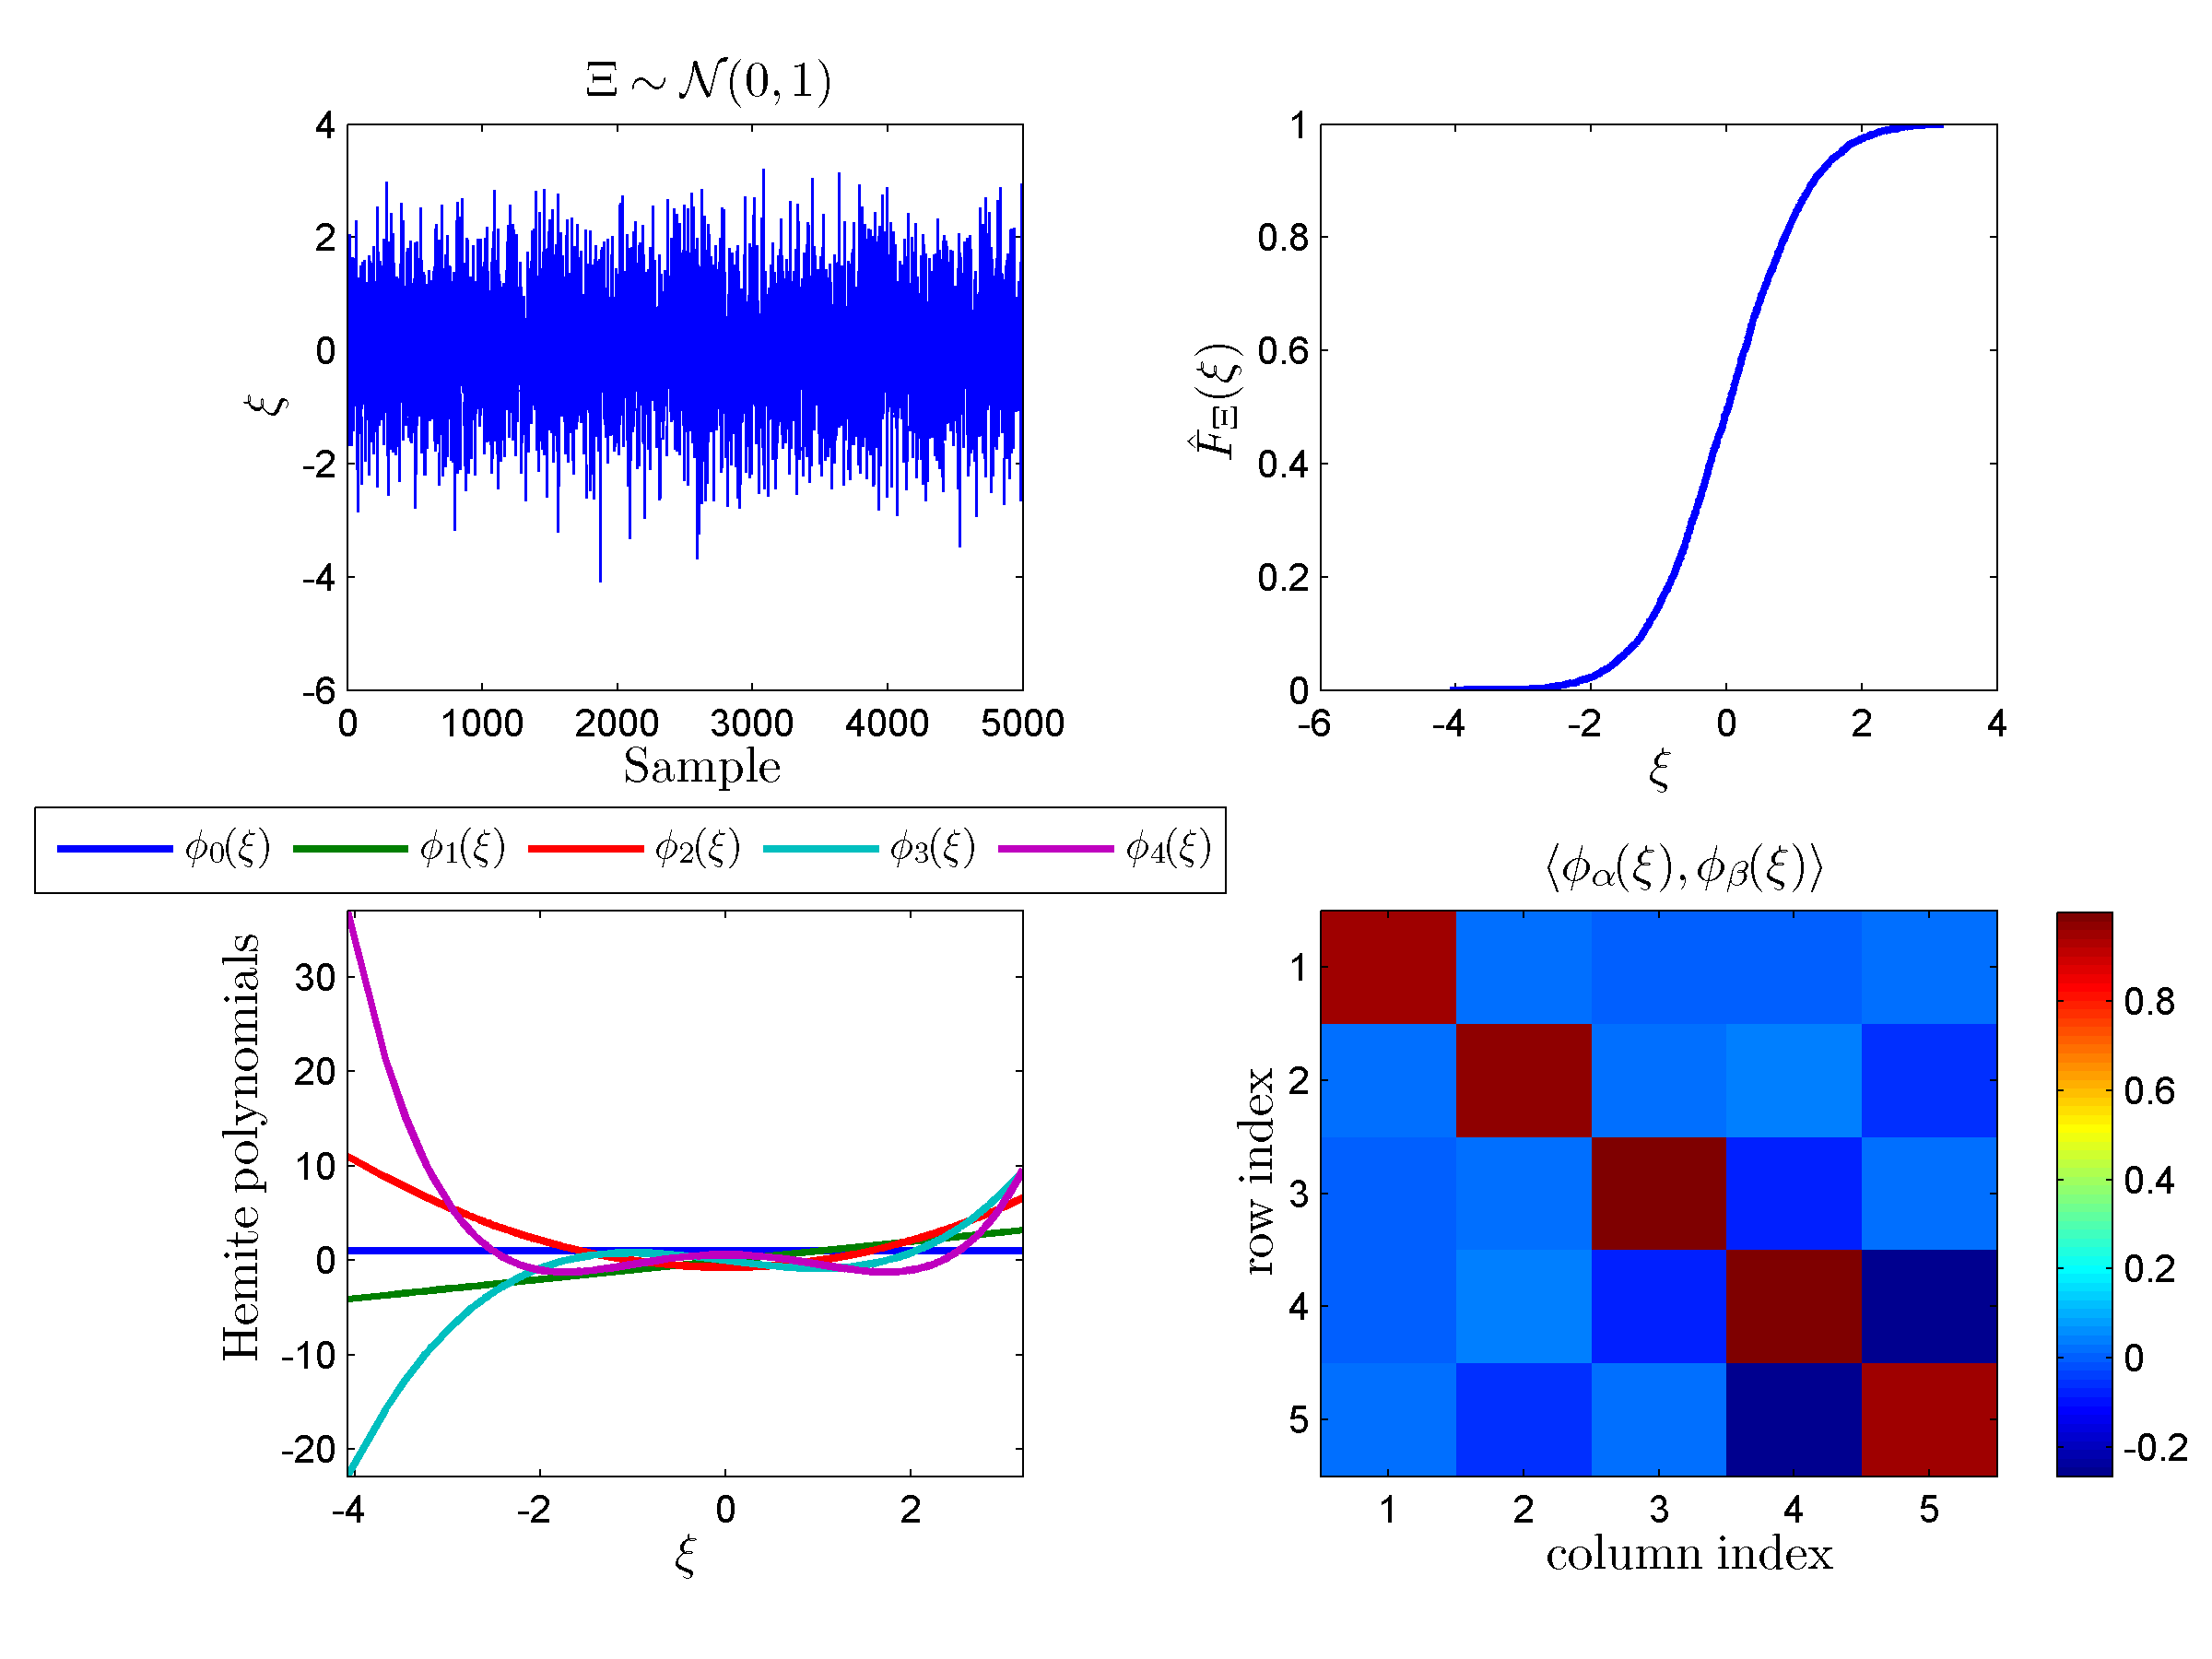
\includegraphics[width=2.9in]{PCbasis.png}
\end{figure}


\end{frame}

\end{document}
